\documentclass[pdf]{prosper}
\usepackage[toc,highlight,linbit,notes,hlsections]{HA-prosper}

\title{The Brainf*ck CPU Project}
\subtitle{An Introduction to \\ FPGA Development using VHDL \\
http://www.clifford.at/bfcpu/}

\author{Clifford Wolf\\
\institution{ROCK Linux - \href{http://www.rocklinux.org}{http://www.rocklinux.org}}\\
\institution{CNGW - \href{http://www.cngw.org}{http://www.cngw.orig}}\\
\institution{LINBIT - \href{http://www.linbit.com}{http://www.linbit.com}}}

\DefaultTransition{Wipe}
\TitleSlideNav{FullScreen}
\NormalSlideNav{ShowBookmarks}
\LeftFoot{\href{http://www.clifford.at}{Clifford Wolf, www.clifford.at} \today}
\RightFoot{ROCK Linux -- CNGW -- LINBIT}


\begin{document}

\maketitle

% ============================================================================

\tsectionandpart{Overview}

\begin{slide}{Building custom hardware}

With programable hardware (such as PLDs and FPGAs) it is possible to
\begin{itemize}
\item Instantly test hardware designs with almost no prototyping costs
\item Simply "upload" hardware designs (bitstream files) to a chip like it would be software
\item Have much fun with building hardware without touching a soldering gun
\end{itemize}

\vspace*{1cm}

With HDLs (such as Verilog and VHDL) it is possible to
\begin{itemize}
\item Describe a hardware design like program source describes the behavior of a program
\item Automatically create bitstream files for different chips from the same (portable) source
\item Simulate the behavior of your hardware on various levels
\end{itemize}

\end{slide}

\begin{slide}{The Brainf*ck CPU}

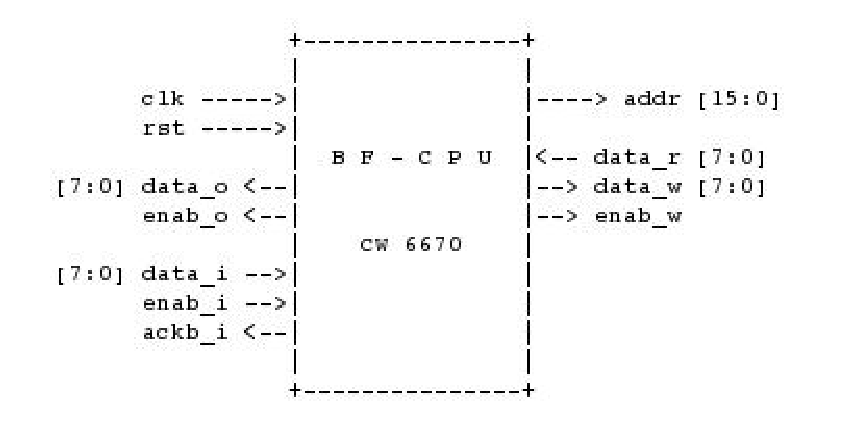
\includegraphics[scale=.80]{schem.eps}

A minimalistic CPU with 8 bit data-bus and 16 bit address-bus which can
execute brainf*ck code. The VHDL design file for it has 260 lines of
code. The optimised variation of the CPU with a 1 byte internal data
cache has 340 lines of code.

\end{slide}

% ============================================================================

\tsectionandpart{Programmable Hardware}

\begin{slide}{PALs}

A PAL is a very simple and limited programable hardware device:\\
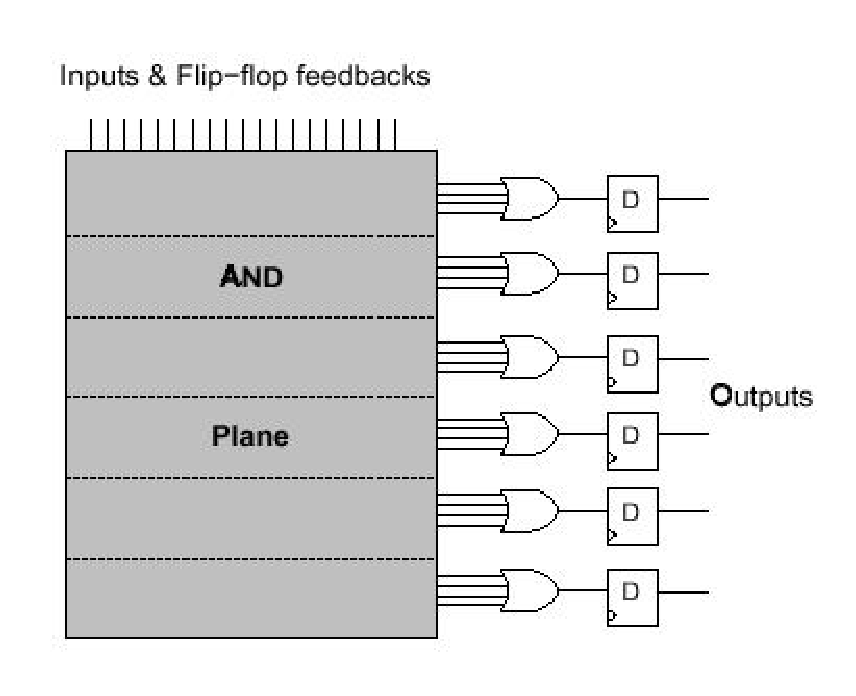
\includegraphics[scale=.50]{pal.eps}

It's programm only consists of a single truth table. Which is implemented
as one big unit with d-flipflops (connected to one global clock) on the
output lines.

\end{slide}

\begin{slide}{PLDs and CPLDs}

A PLD consists of macrocells which are something like better PALs and one
central interconnection logic. PLDs are usually used to connect a high
number of pins with a more or less simple logic at very low cost. Typical
PLD applications are "glue logic" for connecting other ASICS.

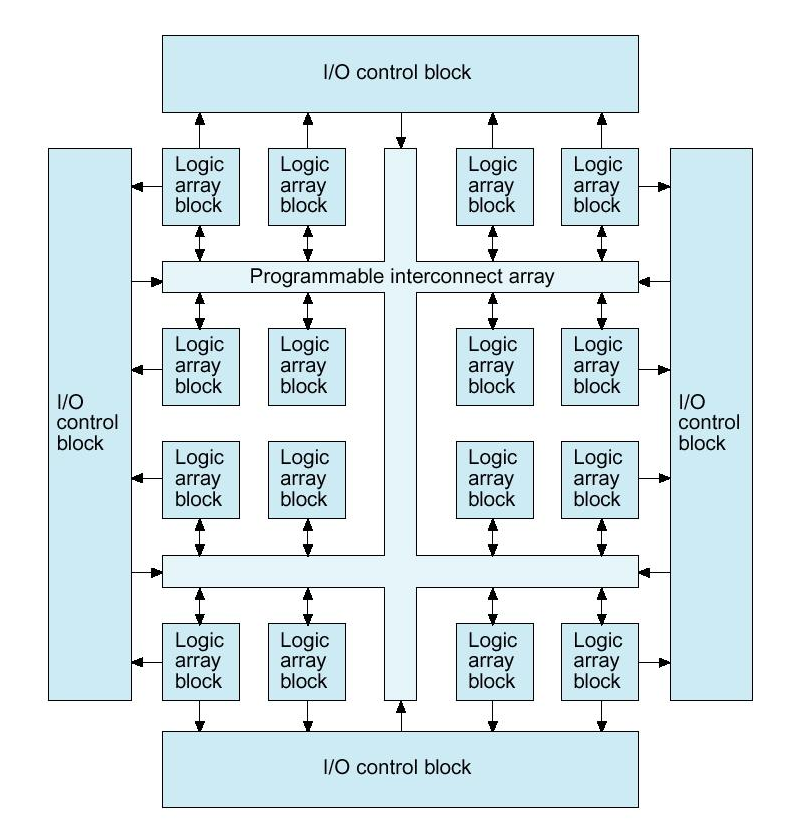
\includegraphics[scale=.45]{cpld.eps}

\end{slide}

\begin{slide}{FPGAs}

FPGAs consist of even more complex logic blocks connected by a very
complex interconnection matrix. FPGAs can implement a very complex logic
on one chip. Typical applications are CPUs and DSPs up to very complex
SoC setups.

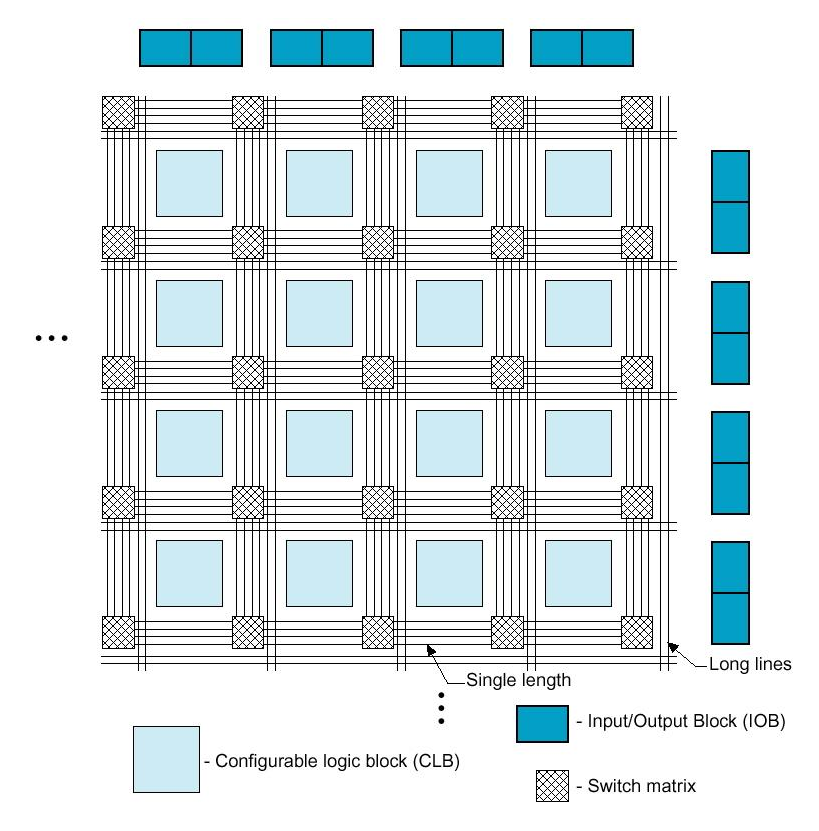
\includegraphics[scale=.40]{fpga.eps}

\end{slide}

\begin{slide}{Recommended reading}
The Xilinx "Detailed Functional Description" Datasheets \\
\vspace*{.5cm}

E.g.: "Spartan-IIE 1.8V FPGA Detailed Functional Description" \\
http://direct.xilinx.com/bvdocs/publications/ds077\_2.pdf

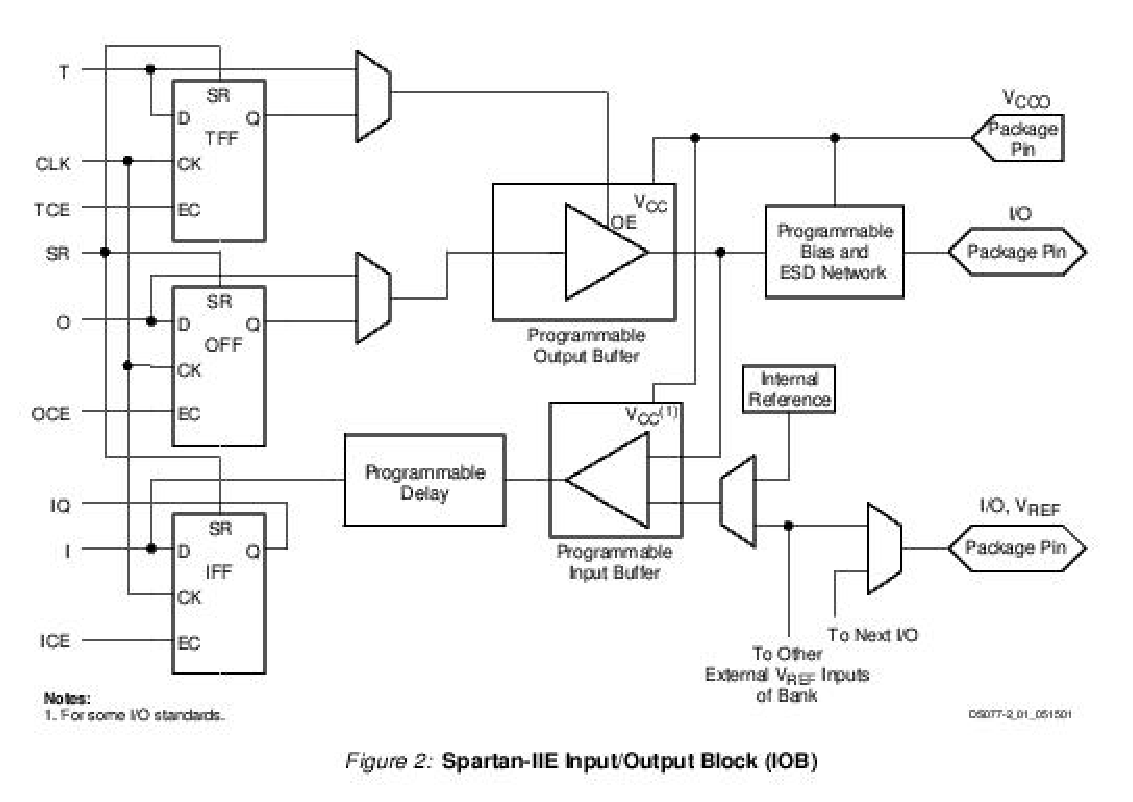
\includegraphics[scale=.50]{xliob.eps}

\end{slide}

% ============================================================================

\tsectionandpart{Introduction to VHDL}

\begin{slide}{What is VHDL}
\begin{itemize}
\item VHDL is the "VHSIC Hardware Description Language"
\vspace*{.3cm}
\item VHSIC is a "Very High Speed Integrated Circuit"
\vspace*{.3cm}
\item VHDL was originally design to document circuits
\vspace*{.3cm}
\item Later on, programs have been developt to generate ciruct designs from VHDL code
\vspace*{.3cm}
\item Only a small subset of correct VHDL code can be used to synthesize designs
\end{itemize}
\end{slide}

\begin{slide}{A 2 bit counter (1)}

A simple clocked 2 bit counter (00, 01, 10, 11, 00, ..):
\begin{itemize}
\vspace*{.3cm}
\item 2 Output signals: D1 (lower bit) and D2 (higher bit)
\vspace*{.3cm}
\item The following truth table shows how to calculate new D1 and D2 from the old values:
\vspace*{.3cm}
\end{itemize}

\begin{verbatim}
 D2  D1  | D2, D1,     D2  D1  | D2,     D1  | D1,
 --------+--------     --------+----     ----+----
  0   0  |  0   1       0   0  |  0       0  |  1
  0   1  |  1   0       0   1  |  1       1  |  0
  1   0  |  1   1       1   0  |  1       0  |  1
  1   1  |  0   0       1   1  |  0       1  |  0

So it turns out:         D2 xor D1         not D1
\end{verbatim}

\end{slide}

\begin{slide}{A 2 bit counter (2)}
The 2 bit counter as circuit:
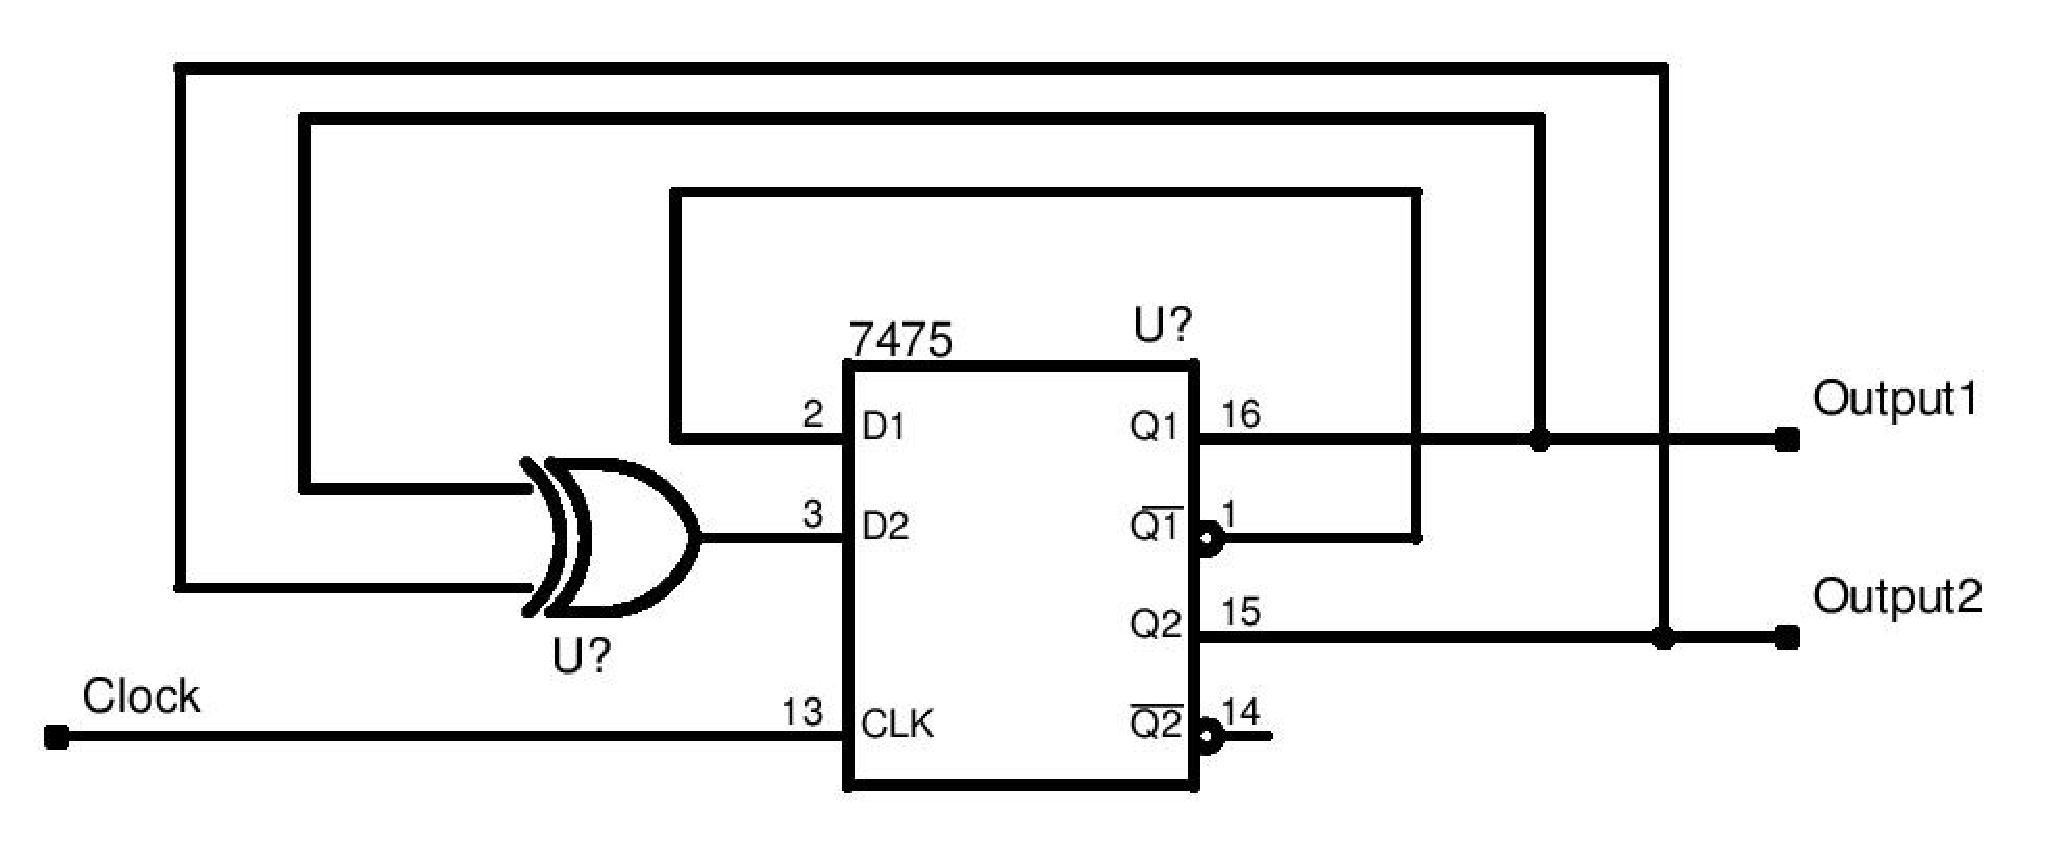
\includegraphics[scale=.25]{bcount.eps}

\vspace*{.3cm}
And this is the VHDL code for the same thing:\\
\begin{verbatim}
        process (clock) begin
            if rising_edge(clock) then
                output1 <= not output1;
                output2 <= output1 xor output2;
            end if;
        end process;
\end{verbatim}

\end{slide}

\begin{slide}{Signals in VHDL}
\begin{itemize}
\item Signals are single wires or buses in the circuit.
\vspace*{.3cm}
\item Buses (multiple wires with one name) are usually called "signal vectors".
\vspace*{.3cm}
\item There are multiple signal types (vitally important: bit and std\_logic).
\vspace*{.3cm}
\item Usually a signal my only have one single source (exception: std\_ulogic).
\vspace*{.3cm}
\item Many signal types have predefined operations (like "xor", "not", "+" or "*").
\vspace*{.3cm}
\item Signals can be assigned a value using the "<=" operator
\end{itemize}
\end{slide}

\begin{slide}{Prozesses in VHDL (1)}
\begin{itemize}

\item Processes are one way to group VHDL statements to a logical unit.
\vspace*{.3cm}
\item A dependency list contains all signals the statements in the process depend on.
\vspace*{.5cm}

\begin{verbatim}
    process (mysignal2, mysignal3) begin
        mysignal1 <= mysignal2 xor mysignal3;
    end process;
\end{verbatim}

\vspace*{.5cm}
\item Clocked processes are the prefered way to use d-flip-flops in the design:

\begin{verbatim}
    process (clk) begin
        if rising_edge(clk) then
                mysignal1 <= mysignal2 xor mysignal3;
        end if;
    end process;
\end{verbatim}

\end{itemize}

\end{slide}

\begin{slide}{Processes in VHDL (2)}
\begin{itemize}
\item Clocked processes may also contain code for reset signals:

\begin{verbatim}
    process (clk, rst) begin
        if rst = '1' then
            mysignal1 <= x"00";
        elsif rising_edge(clk) then
            mysignal1 <= mysignal1 + 1;
        end if;
    end process;
\end{verbatim}

\vspace*{.5cm}
\item Remember: Only a small subset of synthactically and gramatically correct code can actually used to synthesize a real hardware design.
\item No more than one "if rising\_edge(clk)" per process.
\item That "if" must surrond all other instructions in the process.
\item The only allowed variation is the check for a reset signal.

\end{itemize}
\end{slide}

\begin{slide}{Processes in VHDL (3)}
\begin{itemize}
\item Processes may always contain code which implies a feedback of outputs. The first code fragment implies the else-tree of the 2nd one:

\begin{verbatim}
process (clk) begin
        if rising_edge(clk) then
                if enable = 1 then
                        mysignal1 <= mysignal1 + 1;
                end if;
        end if;
end process;

process (clk) begin
        if rising_edge(clk) then
                if enable = 1 then
                        mysignal1 <= mysignal1 + 1;
                else
                        mysignal1 <= mysignal1;
                end if;
        end if;
end process;
\end{verbatim}

\end{itemize}
\end{slide}

\begin{slide}{Variables in VHDL}
\begin{itemize}
\item Variables may be used just as variables in a traditional program.
\item Variables are assigned values using the ":=" operator.
\item Variables are always local to a process.

\begin{verbatim}
process (clk)
        variable temp : std_logic_vector std_logic_vector (15 downto 0);
begin
        if rising_edge(clk) then
                temp := mysignal1;
                temp := temp + 25;
                temp := temp * mysignal2;
                if mysignal3 = '0' then
                        temp := mysignal2;
                end if;
                mysignal1 <= temp;
                temp := temp + 844;
                mysignal2 <= temp;
        end if;
end process;
\end{verbatim}

\end{itemize}
\end{slide}

\begin{slide}{Entities, archs and components}
\begin{itemize}
\item A VHDL project is structured in so-called entities.
\vspace*{.3cm}
\item An "architecture" is the concrete implementation of an entity.
\vspace*{.3cm}
\item An entity may have multiple architectures (e.g. optimized for size or speed).
\vspace*{.3cm}
\item When an entity is used in another entity, it is called a component.
\vspace*{.3cm}
\item Components and signal types can be imported from libraries.
\end{itemize}
\end{slide}

\begin{slide}{VHDL Example (1)}
\begin{verbatim}
library ieee;
use ieee.std_logic_1164.all;
use ieee.numeric_std.all;

entity demo is
        port(
                clk : in std_logic;
                rst : in std_logic;
                dat : out std_logic_vector (15 downto 0);
        );
end demo;
\end{verbatim}
\end{slide}

\begin{slide}{VHDL Example (2)}
\begin{verbatim}
architecture demo_arch of demo is
        signal val : std_logic_vector (15 downto 0);
begin
        process (clk, rst) begin
                if rst = '1' then
                        val <= (others => '0');
                elsif rising_edge(clk) then
                        val <= val + 1;
                end if;
        end process;
        dat <= val;
end demo_arch;
\end{verbatim}
\end{slide}

\begin{slide}{The Brainf*ck CPU}
[ Discussion the Brainf*ck CPU VHDL code ]
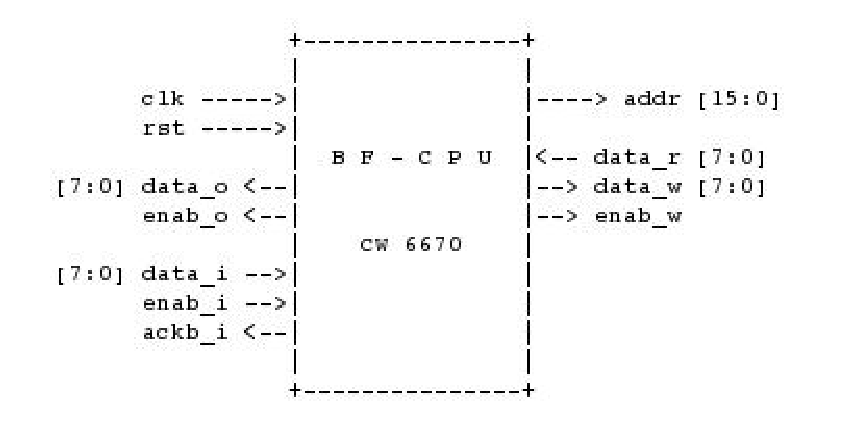
\includegraphics[scale=.80]{schem.eps}
\end{slide}

\begin{slide}{Credits}
\begin{itemize}

\item LINBIT Information Technologies GmbH: \\
http://www.linbit.com/
\vspace*{.5cm}

\item The ROCK Linux Project: \\
http://www.rocklinux.org/
\vspace*{.5cm}

\item Clifford Wolf: \\
http://www.clifford.at/
\vspace*{.5cm}

\end{itemize}

\vspace*{1.5cm}\hspace*{2cm}
http://www.clifford.at/bfcpu/

\end{slide}


\end{document}

